\documentclass[a4paper,11pt]{report}
\usepackage[spanish,mexico]{babel}
\usepackage[utf8]{inputenc}
\usepackage[T1]{fontenc}
\usepackage{amsmath,bm}
\usepackage{enumitem}
\usepackage{amssymb}
\usepackage{wasysym}
\usepackage[dvipsnames,pdftex]{color}
\usepackage[x11names]{xcolor}
\usepackage{tikz, tkz-euclide}
\usepackage[american]{circuitikz}
\usepackage{siunitx}
\usetikzlibrary{arrows}
\usepackage{textcomp}
\usepackage[colorinlistoftodos]{todonotes}
%\usepackage[left=2cm,right=1.5cm,top=1cm,bottom=1cm]{geometry}
%\usepackage{helvet}
%\renewcommand{\familydefault}{\sfdefault}
\setlength{\oddsidemargin}{0in}
\usepackage{geometry}
\geometry{total = {180mm,270mm},
			left = 20mm, top = 20mm,
            right=10mm,bottom=20mm,%
            footskip=10mm}
\usepackage{float} 
% \setlength{\topmargin}{0in}
% \setlength{\voffset}{-0.5in}
% \setlength{\hoffset}{0.3in}
% \setlength{\textheight}{700pt}
% \setlength{\textwidth}{440pt}
% \setlength{\topskip}{0in}
% \setlength{\parskip}{2ex}
 \renewcommand{\baselinestretch}{1.2}
\usepackage{diagbox}
\usepackage{array}
\usepackage{listings}
\usepackage{caption}
%%% comandos definidos por el usuario
\begin{document}
\setcounter{page}{1}
\pagenumbering{roman}
\thispagestyle{empty}
\begin{center}
{\huge UNIVERSIDAD NACIONAL DE INGENIERÍA}\\[0.9cm]
{\Large FACULTAD DE INGENIERÍA MECÁNICA}\\[0.6in]
\end{center}
\begin{figure}[h]
\begin{center}

\includegraphics[scale=0.33]{logoUNI.png}
\vspace{0cm}
\end{center}
\end{figure}
\vspace{0.5cm}
\begin{center}
INFORME DE LABORATORIO\\
LABORATORIO DE CIRCUITOS ELÉCTRICOS\\[5mm]
{\large TEOREMAS DE THEVENIN, NORTON Y MÁXIMA POTENCIA DE TRANSFERENCIA}\\[10mm]
\vfill
LIMA - PERÚ \hfill SEPTIEMBRE 2019
\end{center}
\newpage
\thispagestyle{empty}
\begin{center}
{\Huge TEOREMAS DE THEVENIN, NORTON Y MÁXIMA POTENCIA DE TRANSFERENCIA}\\[0.7cm]
\small ENTREGADO:\\[0.05cm]
\small 25 SEPTIEMBRE 2019\\[1.2cm]
\end{center}
\begin{flushleft}
{\large ALUMNO:}\\[2cm]
\end{flushleft}
%\begin{center}
%\begin{tabular}{c@{\hspace{0.5in}}c}
%\rule[1pt]{3.14in}{1pt}\\
%Sotelo Cavero Sergio, 20172125K% & Nombre 5, 2017 \\[1.5cm]
%\end{tabular}
%\end{center}
\begin{center}
\begin{tabular}{c@{\hspace{0.6in}}c}
\rule[1pt]{3.14in}{1pt}\\
Huaroto Villavicencio Josué, 20174070I \\[2cm]
\rule[1pt]{3.14in}{1pt}\\
Landeo Sosa Bruno, 20172024J \\[2cm]
\rule[1pt]{3.14in}{1pt}\\
Quesquén Vitor Angel, 20170270C \\[2cm]
\rule[1pt]{3.14in}{1pt}\\
Sotelo Cavero Sergio, 20172125K \\[2cm]
\end{tabular}
\end{center}
%\begin{center}
%\begin{tabular}{c}
%\rule[1pt]{3.14in}{1pt}\\
%Huaroto Villavicencio Josué, 20174070I \\[2.5cm]
%\end{tabular}
%\end{center}

%\rule[1pt]{3.14in}{1pt}\\
%Maguiña Amaya Wladimir, 20172019F \\[3cm]
%\rule[1pt]{3.14in}{1pt}\\
%Luis Sosa Jose, 19774147I \\[3cm]
%\rule[1pt]{3.14in}{1pt}\\
%Sotelo Cavero Sergio, 20172125K
%\end{tabular}
%\end{center}
%\\[0.7cm]
{\large PROFESOR:} \\[2cm]
\begin{center}
\begin{tabular}{c}
\rule[3pt]{4.8in}{1pt}\\[1pt]
ING. SINCHI YUPANQUI, FRANCISCO 
\end{tabular}
\end{center}
\vfill
%\newpage
%\begin{center}
%{\Large \bf{RESUMEN}}
%\end{center}
\newpage
\tableofcontents
%\listoffigures
%\addcontentsline{toc}{chapter}{Índice de figuras}
\newpage
\pagenumbering{arabic} %%% esto es para regresar el modo de numeración a numeración arábiga
\setcounter{page}{1}  %%% empezamos en página 1
%\part{Introducción}
\chapter{Objetivos}
\begin{enumerate}
\item Tomar en consideración las medidas de seguridad indicadas para la realización de un buen trabajo en el laboratorio.
\item Verificar experimentalmente los teoremas de Thevenin y Norton y  maxima potencia eléctrica.
\item Conocer mejor nuestro laboratorio de circuitos y sus alcances mediante esta experiencia.
\end{enumerate}
\chapter{Marco teórico}
\section{Teorema de Thevenin}
El teorema de Thévenin establece que si una parte de un circuito eléctrico lineal está comprendida entre dos terminales A y B, esta parte en cuestión puede sustituirse por un circuito equivalente que esté constituido únicamente por un generador de tensión en serie con una resistencia, de forma que al conectar un elemento entre los dos terminales A y B, la tensión que queda en él y la intensidad que circula son las mismas tanto en el circuito real como en el equivalente.\\
El teorema de Thévenin fue enunciado por primera vez por el científico alemán Hermann von Helmholtz en el año 1853, pero fue redescubierto en 1883 por el ingeniero de telégrafos francés Léon Charles Thévenin, de quien toma su nombre.
\subsection{Cálculo de la tensión de Thevenin}
Para calcular la tensión de Thévenin, $V_{th}$, se desconecta la carga (es decir, la resistencia de la carga) y se calcula $V_{AB}$. Al desconectar la carga, la intensidad que atraviesa $R_{th}$ en el circuito equivalente es nula y por tanto la tensión de $R_{th}$ también es nula, por lo que ahora $V_{AB} = V_{th}$ por la segunda ley de Kirchhoff.
Debido a que la tensión de Thévenin se define como la tensión que aparece entre los terminales de la carga cuando se desconecta la resistencia de la carga también se puede denominar tensión en circuito abierto.\\
Para calcular la resistencia de Thévenin, se desconecta la resistencia de carga, se cortocircuitan las fuentes de tensión y se abren las fuentes de corriente. Se calcula la resistencia que se ve desde los terminales $AB$ y esa resistencia $R_{AB}$ es la resistencia de Thevenin buscada $R_{th} = R_{AB}$.
\section{Teorema de Norton}
Establece que cualquier circuito lineal se puede sustituir por una fuente equivalente de corriente en paralelo con una impedancia equivalente. Al sustituir un generador de corriente por uno de tensión, el borne positivo del generador de tensión deberá coincidir con el borne positivo del generador de corriente y viceversa. 
\subsection{Cálculo del Norton Equivalente}
El circuito Norton equivalente consiste en una fuente de corriente $I_{No}$ en paralelo con una resistencia $R_{No}$. Para calcularlo:
\begin{enumerate}
\item Se calcula la corriente de salida, $I_{AB}$, cuando se cortocircuita la salida, es decir, cuando se pone una carga (tensión) nula entre $A$ y $B$. Al colocar un cortocircuito entre $A$ y $B$ toda la intensidad $I_{No}$ circula por la rama $AB$, por lo que ahora $I_{AB}$ es igual a $I_{No}$.
\item Se calcula la tensión de salida, $V_{AB}$, cuando no se conecta ninguna carga externa, es decir, cuando se pone una resistencia infinita entre $A$ y $B$. $R_{No}$ es ahora igual a $V_{AB}$ dividido entre $I_{No}$ porque toda la intensidad $I_{No}$ ahora circula a través de $R_{No}$ y las tensiones de ambas ramas tienen que coincidir ( $V_{AB} = I_{\mathrm{No}}R_{\mathrm{No}}$).
\end{enumerate}
\section{Teorema de máxima potencia}
El teorema establece cómo escoger (para maximizar la transferencia de potencia) la resistencia de carga, una vez que la resistencia de fuente ha sido fijada, no lo contrario. No dice cómo escoger la resistencia de fuente, una vez que la resistencia de carga ha sido fijada. Dada una cierta resistencia de carga, la resistencia de fuente que maximiza la transferencia de potencia es siempre cero, independientemente del valor de la resistencia de carga.\\
Para alcanzar la máxima eficiencia, la resistencia de la fuente (sea una batería o un dínamo) debería hacerse lo más pequeña posible. Bajo la luz de este nuevo concepto, obtuvieron una eficiencia cercana al 90\% y probaron que el motor eléctrico era una alternativa práctica al motor térmico. En esas condiciones la potencia disipada en la carga es máxima y es igual a: 
$$
P_{max} = \frac{V^{2}}{4R_{g}}
$$
\chapter{Cuestionario}
\section{Parte 1}
\begin{enumerate}[label=\arabic*),font=\bfseries]
\item \textbf{Hacer un diagrama del circuito usado, indicando las mediciones efectuadas en la carga en los pasos 1, 2, y 3.}
\begin{figure}[H]
\begin{center}
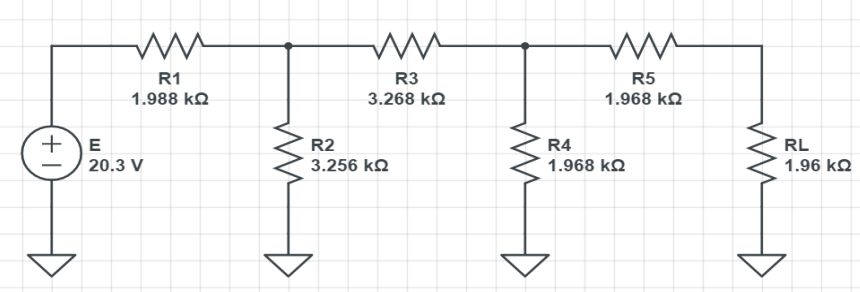
\includegraphics[scale=0.45]{1,1,1.png}
\caption{Circuito 1}
\end{center}
\end{figure}
\begin{figure}[H]
\begin{center}
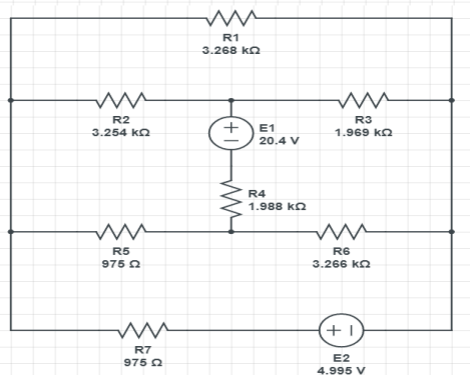
\includegraphics[scale=0.5]{1,1,2.png}
\caption{Circuito 2}
\end{center}
\end{figure}
\item \textbf{Con las mediciones efectuadas armar el circuito de Thevenin y Norton equivalentes y verificar la tensión y corriente de  carga. Explicar los errores que se puede tener.}
\begin{figure}[H]
\centering
\begin{tikzpicture}[draw=DeepSkyBlue4,thin]
\tkzDefPoints{	0/0/A,
0/4/B,
3/4/C,
3/0/D,
7/4/E,
8/4/F,
8/0/G,
10/-0.5/H}
\draw[draw opacity=0, fill=yellow!30] (0,2) circle (.4);
\draw ({8,4}) to[R = 3.356\si{\kohm},color=Aquamarine4] (B) to[V=3.895V,color=red,thin] (A);
%\draw (C) to[R = 3.256\si{\kohm},color=Aquamarine4] (D);
\draw (A) to ({8,0});
\draw ({8,0}) to[R=$R_{L}$,color=Aquamarine4] ({8,4});
%\draw (D) to ({10,0});
%\draw (C) to[R = 3.268\si{k\ohm},color=Aquamarine4] (E);
%\draw (E) to[R = 1.962\si{k\ohm},color=Aquamarine4] ({7,0});
%\draw (E) to[R = 1.968\si{\kohm},color=Aquamarine4] ({10,5});
%\draw ({10,5}) to[R = 3.366\si{\kohm},color=Aquamarine4] ({10,0});
%\draw (F) to[R = 193.3\si{\ohm},color=Aquamarine4] (G);
%\draw (G) to ({10,0});
%\draw ({10,0}) to (H) node[sground]{};
\end{tikzpicture}
\end{figure}
\begin{figure}[H]
\centering
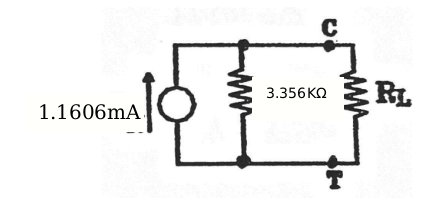
\includegraphics[scale=0.65]{sergod.png}
\end{figure}
Hallando la tensión y corriente de carga:
$$
V_{L} = \frac{3.825}{(3.334+1.96)\cdot 10^{3}}\cdot 1.96\cdot 10^{3} = 1.436 \mathrm{V} \longrightarrow I_{L} = 0.7326\,\mathrm{mA}
$$
En el laboratorio se midió un voltaje de carga de $V_{L} = 1.623$V. El error sería:
$$
\%\,\mathrm{Error} = \frac{1.623-1.436}{1.623}\cdot 100\% = 11.52187\% 
$$
Este error es menor pues es de medición directa, no implicó otras resistencias que propaguen más el error como en el caso donde se obtendrá el voltaje de carga por la reducción de las mismas.\\
Thevenin medido equivalente:
\begin{figure}[H]
\centering
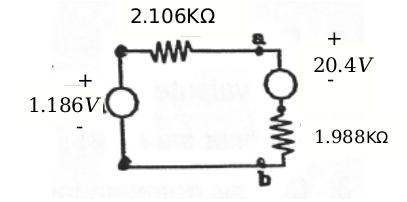
\includegraphics[scale=0.65]{sergod2.png}
\end{figure}
Norton equivalente:
\begin{figure}[H]
\centering
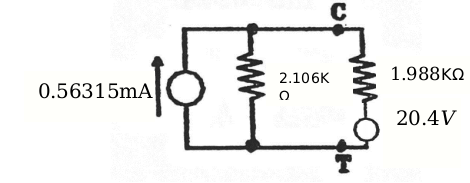
\includegraphics[scale=0.65]{sergod3.png}
\end{figure}
Hallando la tensión y corriente de carga:
$$
V_{L} = \frac{1.186-20.4}{(2.106+1.988)\cdot 10^{3}}\cdot 1.9888\cdot 10^{3} + 20.4 = 11.06989\,\mathrm{V}
$$
Es decir, se verifican los teoremas. $I_{L} = 0.7326\,$mA. En el laboratorio se midió un voltaje de carga de $V_{L} = 10.663\,$V.\\
El error de voltaje de carga de Thevenin medido respecto al teórico es:
$$
\%\,\mathrm{Error} = \frac{11.06989-10.663}{10.663}\cdot 100\% = 3.81\% 
$$
Los errores son muy aceptables, sobre todo en el segundo circuito lo que nos hace comprobar la eficiencia de los teoremas de Thevenin y Norton, que son muy efectivos y a partir de ahora podremos utilizarlos de manera gradual y más confiable gracias a esta experiencia práctica.
\item \textbf{Con los datos de las resistencias medidas, hallar las incógnitas de RL en forma directa. Hallar teóricamente el circuito Thevenin y Norton, verificando los teoremas propuestos. Explicar las posibles causas de error.}\\
Del circuito 1:
\begin{figure}[H]
\centering
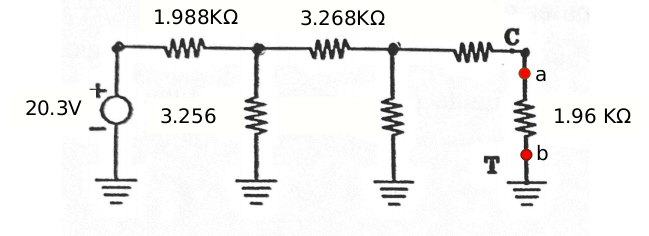
\includegraphics[scale=0.6]{lan1.png}
\end{figure}
Hallando la tensión y corriente de carga teóricamente de forma directa:
\begin{figure}[H]
\centering
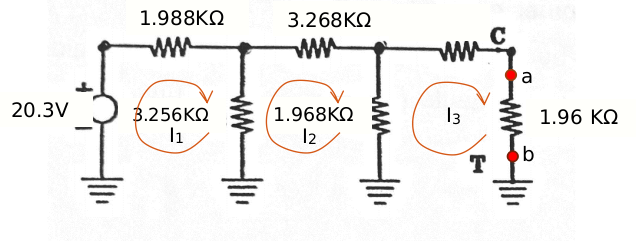
\includegraphics[scale=0.6]{lan2.png}
\end{figure}
$$
\begin{bmatrix}
20.3 \\
0 \\
0 \\
\end{bmatrix} = 10^{3} \cdot \begin{bmatrix}
5.244 & -3.2556 & 0 \\
-3.256 & 8.485 & -1.962 \\
0 & -1.962 & 5.89 \\
\end{bmatrix} \cdot \begin{bmatrix}
I_{1} \\
I_{2} \\
I_{3}
\end{bmatrix} \rightarrow I_{1} = 5.2179, I_{2} = 2.169, I_{3} = 0.7225\,(\mathrm{mA})
$$
La corriente de la carga es \fbox{0.7225\,mA} y el voltaje de carga es \fbox{1.41619\,V}.\\
Hallando teóricamente Thevenin y Norton.
\begin{figure}[H]
\centering
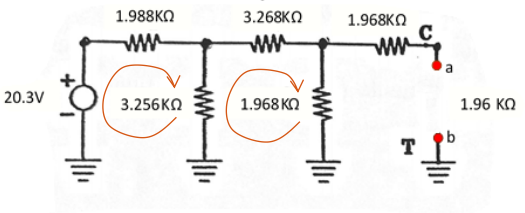
\includegraphics[scale=0.6]{lan3.png}
\end{figure}
Aplicando la ley de mallas de Kirchhoff:
$$
\begin{bmatrix}
20.3 \\
0 \\
\end{bmatrix} = \begin{bmatrix}
-5.244 & 3.2556 \\
3.256 & -8.485 \\
\end{bmatrix} \cdot \begin{bmatrix}
I_{1} \\
I_{2}
\end{bmatrix} \rightarrow I_{1} = -5.082, I_{2} = -1.9498\,(\mathrm{mA})
$$
$$
E_{th} = I_{2}\cdot (1.962) = -3.825\,\mathrm{V} \longrightarrow I_{No} = 1.1606\,\mathrm{mA}
$$
Y al transformar el circuito a pasivo y reducir, se obtiene una resistencia equivalente entre bornes $a$ y $b$:
\begin{figure}[H]
\centering
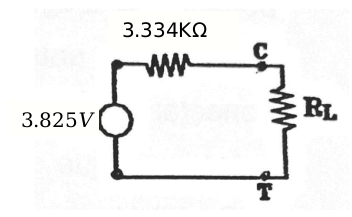
\includegraphics[scale=0.6]{lan4.png}
\end{figure}
\begin{figure}[H]
\centering
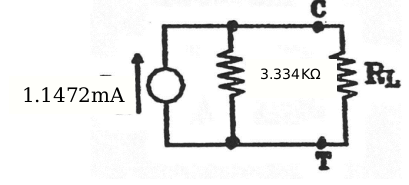
\includegraphics[scale=0.6]{lan5.png}
\end{figure}
Hallando la tensión y corriente de carga:
$$
V_{L} = \frac{3.825}{(3.334 + 1.96)\cdot 10^{3}}\cdot 1.96\cdot 19^{3} = 1.41619\,\mathrm{V}
$$
Es decir, se verifican los teoremas.\\
En el laboratorio se midió un voltaje de carga de: 1.623\,V. El error viene dado por:
$$
\%\mathrm{Error} = \frac{1.623 - 1.416}{1.623}\cdot 100\% = 12.754\%
$$
Con un error de 12.754\% es aceptada la medición. Hay muchas variables que afectan el error de medición, entre ellas podemos afirmar que los instrumentos de medición tienen un ligero error propio, además existieron factores medio ambientales tales que pudieron afectar la medición, así como las ligeras resistencias de los cables al unir las resistencias, aunque estas son mínimas, se consideran como pérdidas.\\
Del circuito 2:
\begin{figure}[H]
\centering
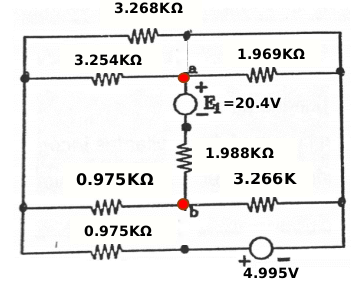
\includegraphics[scale=0.6]{lan6.png}
\end{figure}
Hallando la tensión y corriente de carga teóricamente de forma directa:
\begin{figure}[H]
\centering
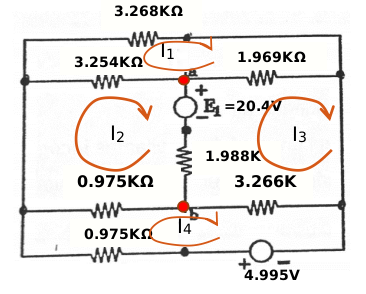
\includegraphics[scale=0.6]{lan7.png}
\end{figure}
\begin{align*}
\begin{bmatrix}
3.268+3.254+1.969 & -3.254 & -1.969 & 0 \\
-3.254 & 3.254+0.975+1.988 & -1.988 & -0.975 \\
-1.969 & -1.988 & 1.988+1.969+3.266 & -3.266 \\
0 & -0.975 & -3.266 & 0.975+0.975+3.266 \\
\end{bmatrix} &\cdot \begin{bmatrix}
I_{1} \\
I_{2} \\
I_{3} \\
I_{4}
\end{bmatrix}\\
&=\begin{bmatrix}
0\\
-20.4 \\
20.4 \\
4.995 \\
\end{bmatrix}
\end{align*}
$$
I_{1} = 0.52775, \hspace{10pt} I_{2} = -1.14581, \hspace{10pt} I{3} = 4.169, \hspace{10pt} I_{4} = 3.354 \, (\mathrm{mA})
$$
Y la corriente de carga es $I_{3} - I_{2} = 5.31562\,$mA. Mientras que el voltaje de carga es 9.83326\,V.
Hallando teóricamente Thevenin y Norton:
\begin{figure}[H]
\centering
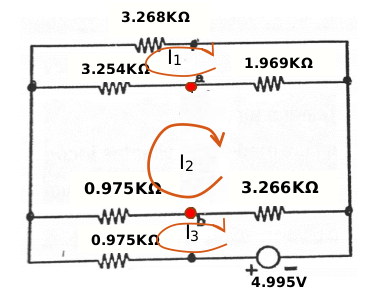
\includegraphics[scale=0.6]{lan8.png}
\end{figure}
Del circuito pasivo, reduciendo paralelos, y haciendo un cambio de delta a estrella se obtiene la resistencia equivalente:
$$
R_{eq} = 1.77883\,\mathrm{k}\Omega
$$
Aplicando la ley de las mallas de Kirchhoff:
$$
\begin{bmatrix}
0\\
0 \\
4.995 \\
\end{bmatrix} =  \begin{bmatrix}
3.268+3.254+1.969 & -3.254-1.969 & 0 \\
-3.254-1.969 & 3.254+1.969+0.975+3.266 & -0.975-3.266 \\
0 & -0.975-3.266 & 0.975+3.266+0.975 \\
\end{bmatrix} \cdot \begin{bmatrix}
I_{1} \\
I_{2} \\
I_{3}
\end{bmatrix}
$$
$$
I_{1} = 0.89127, \hspace{10pt} I_{2} = 1.44893, \hspace{10pt} I{3} = 2.13572 \, (\mathrm{mA}) \longrightarrow I_{No} = 0.6436\,\mathrm{mA}
$$
Thevenin teórico:
\begin{figure}[H]
\centering
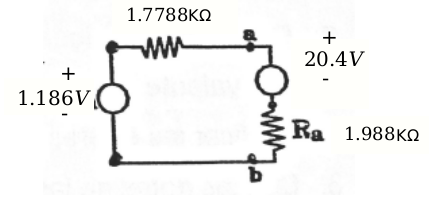
\includegraphics[scale=0.6]{lan9.png}
\end{figure}
Norton teórico:
\begin{figure}[H]
\centering
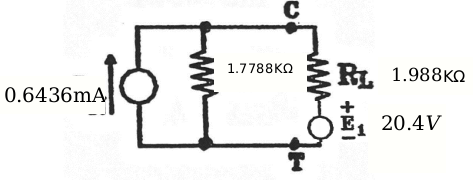
\includegraphics[scale=0.6]{lan10.png}
\end{figure}
Hallando la tensión y corriente de carga:
$$
V_{L} = \frac{1.14-20.59}{(1.7+1.97)\cdot 10^{3}}\cdot 1.99\cdot 10^{3} + 20.4 = 9.805844\,\mathrm{V}
$$
Es decir, se verifican los teoremas. En el laboratorio se midió un voltaje de carga de 10.663\,V. El error sería:
$$
\%\,\mathrm{Error} = \frac{10.663-9.805}{10.663}\cdot 100\% = 8.046\%
$$
La aclaración de los errores es la misma del circuito anterior, aquí se aprecia cierto grado de perfeccionamiento en nuestras mediciones.
\item \textbf{Investigar sobre las limitaciones para aplicar los teoremas de Thevenin y Norton en Circuitos Eléctricos.}\\
\begin{itemize}
\item Una de las limitaciones que se tienen al aplicar el teorema de Thevenin o Norton es que la red en la cual se va aplicar debe ser lineal; es decir debe cumplir 2 condiciones para verificar si los elementos del circuito son lineales. La primera es la condición de homogeneidad y la segunda condición es la aditiva.\\
La propiedad de homogeneidad se cumple cuando a la entrada le multiplicamos por un factor, entonces nuestra salida también quedara multiplicada por este factor.\\
A continuación, vamos a analizar una resistencia y verificar si se cumplen las 2 condiciones, teniendo en cuenta que se cumple la ley de ohm.
$$
V = IR
$$
Al multiplicar por el factor $k$ nos queda:
$$
kV = kIR
$$
Entonces se dice que la propiedad de homogeneidad se cumple.\\
La propiedad de aditiva nos dice que la suma de 2 entradas ($i_{1}+i_{2}$) va a darnos una respuesta igual a la suma de valores de las respuestas ($v_{1} + v_{2}$) donde cada respuesta se obtiene aplicando por separado a cada entrada, con base a la relación tensión corriente obtenido de la ley de ohm.
$$
v_{1} = i_{1}R \hspace{20pt} v_{2} = i_{2}R \longrightarrow v_{1} + v_{2} = (i_{1} + i_{2})R
$$
Entonces se cumple la propiedad aditiva. En conclusión, podemos decir que un resistor es lineal a causa de la ley de ohm. En general un circuito lineal constaría de elementos lineales, fuentes lineales dependientes e independientes.
\item Otra desventaja que se presenta es cuando nos encontramos en la situación en donde un circuito dependiente, la red principal contiene a la fuente dependiente y la otra red este la variable independiente de la que depende la fuente y también ocurre la misma limitación en el caso contrario; es decir no vamos a poder separar la fuente dependiente de su respectiva variable independiente.
\end{itemize}
\item \textbf{Busque algunas aplicaciones de los teoremas Thevenin y Norton y explicar las ventajas que ofrecen.}\\
En los sistemas eléctricos grandes, por ejemplo, se suele utilizar la reducción de Thevenin para el cálculo de corrientes máximas en condiciones de falla (cortocircuitos) en las redes (y así calcular y coordinar sus protecciones), ya que podemos representar a todo el sistema de un país con una simple fuente de voltaje con una impedancia en serie. Sin el teorema de Thevenin sería muy difícil predecir el comportamiento de un sistema en condiciones de falla y no existiría la coordinación, si fallara un elemento del circuito, sin estos teoremas, se debería dejar afuera todo el sistema. En adición a esto, el teorema Norton es muy usado para cálculos eficientes de nodos o puntos circuitales, así como la prueba efectiva de componente por componente de redes y circuitos interconectados.
\item \textbf{¿Cómo se puede aplicar los teoremas de Thevenin y Norton en circuitos que presenten fuentes controladas?}\\
Para la resolución de este tipo de circuitos, primero tenemos que hallar el  o , que tienen el mismo valor, entonces tenemos que poner todas las fuentes de voltaje independientes  en cortocircuito y las de corriente en circuito abierto, además las fuentes que son dependientes se las dejan tal como están.\\
Hecho esto debemos poner  entre los bornes una fuente de corriente o una fuente de voltaje, y entonces $R_{th} = v_{o}/i_{o}$ donde $v_{o}$ es el potencial entre los bornes de la fuente de corriente o el potencial de la fuente de voltaje que hemos agregado, y $i_{o}$ sería la intensidad de la fuente de corriente o la corriente que pasa por la fuente de voltaje. Resolvemos el circuito para hallar cualquiera de los 2 valores que nos falten para hallar el $R_{th}$.\\
Cabe resaltar que si $R_{th}$ es negativo significa que la fuente dependiente suministra potencia al circuito y por consiguiente podremos representar el equivalente como una resistencia negativa.
\begin{center}
\begin{picture}(180,90)
\put(0,0){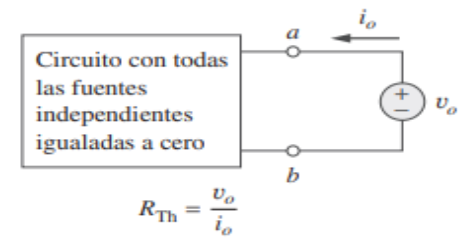
\includegraphics[scale=0.4]{1,6.png}}
\put(143,87){\colorbox{white}{$i_{o}$}}
\put(110,82){\colorbox{white}{$a$}}
\put(110,21){\colorbox{white}{$b$}}
\put(174,54){\colorbox{white}{$v_{o}$}}
\put(45,8){\colorbox{white}{$\displaystyle R_{th} = \frac{v_{o}}{i_{o}}$}}
\end{picture}
\end{center}
Finalmente hallamos el $V_{th}$ o el $I_{N}$, para hallar el primero se procede a resolver la parte del circuito principal tal como está sin volverlo pasivo y así poder  hallar el potencial entre los bornes en el queremos analizar. Para el segundo solo se halla la corriente que pasa entre los bornes a analizar, al cortocircuitar esos bornes.
\end{enumerate}
\section{Parte 2}
\begin{enumerate}[label=\arabic*),font=\bfseries, style=nextline]
\item \textbf{Hacer un diagrama del circuito utilizado y en un cuadro aparte, dar los valores de $\bm{V_{L}}$ e $\bm{I_{L}}$ obtenidos por medición directa, y el correspondiente valor de $\bm{R_{L}}$ determinado indirectamente.}
\begin{figure}[H]
\begin{center}
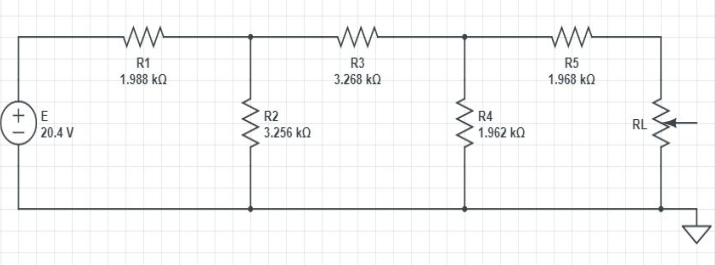
\includegraphics[scale=0.45]{2,1.png}
\end{center}
\end{figure}
\item \textbf{En la misma tabla indicar el valor de potencia $\bm{P_{L}}$, que se consume en $\bm{R_{L}}$ y $\bm{P}$ que entrega la fuente, en cada caso de los determinados anteriormente.}
\begin{center}
\begin{tabular}{|c|c|c|c|}
\hline 
$V_{L}$ (V) & $I_{L}$ (mA) & $R_{L}$ (k$\Omega$) & $P_{L}$ (mW) \\ 
\hline 
0.074 & 1.12121 & 0.066 & 0.083 \\ 
\hline 
0.88 & 0.88 & 1 & 0.7744 \\ 
\hline 
1.623 & 0.6828 & 2.377 & 1.1082 \\ 
\hline 
1.9 & 0.5938 & 3.2 & 1.1281 \\ 
\hline 
1.94 & 0.5739 & 3.38 & 1.1135 \\ 
\hline 
2.393 & 0.4351 & 5.5 & 1.0412 \\ 
\hline 
2.433 & 0.42684 & 5.7 & 1.0385 \\ 
\hline 
2.847 & 0.3006 & 9.47 & 0.8559 \\ 
\hline 
2.952 & 0.26934 & 10.96 & 0.7951 \\ 
\hline
\end{tabular}
\end{center}
El $R_{eq}$ según las mediciones es de 3.356\,k$\Omega$.
\item \textbf{Graficar $\bm{P_{L} \, \mathrm{vs} \, R_{L}}$, para determinar gráficamente el valor de $\bm{R_{L}}$ con el que se obtiene el valor de la resistencia de carga que absorbe la máxima potencia.}
%\begin{figure}[H]
%\centering
%\def\svgwidth{12cm}
%\input{kskenPDF.pdf_tex}
%\end{figure}
\begin{figure}[H]
\centering
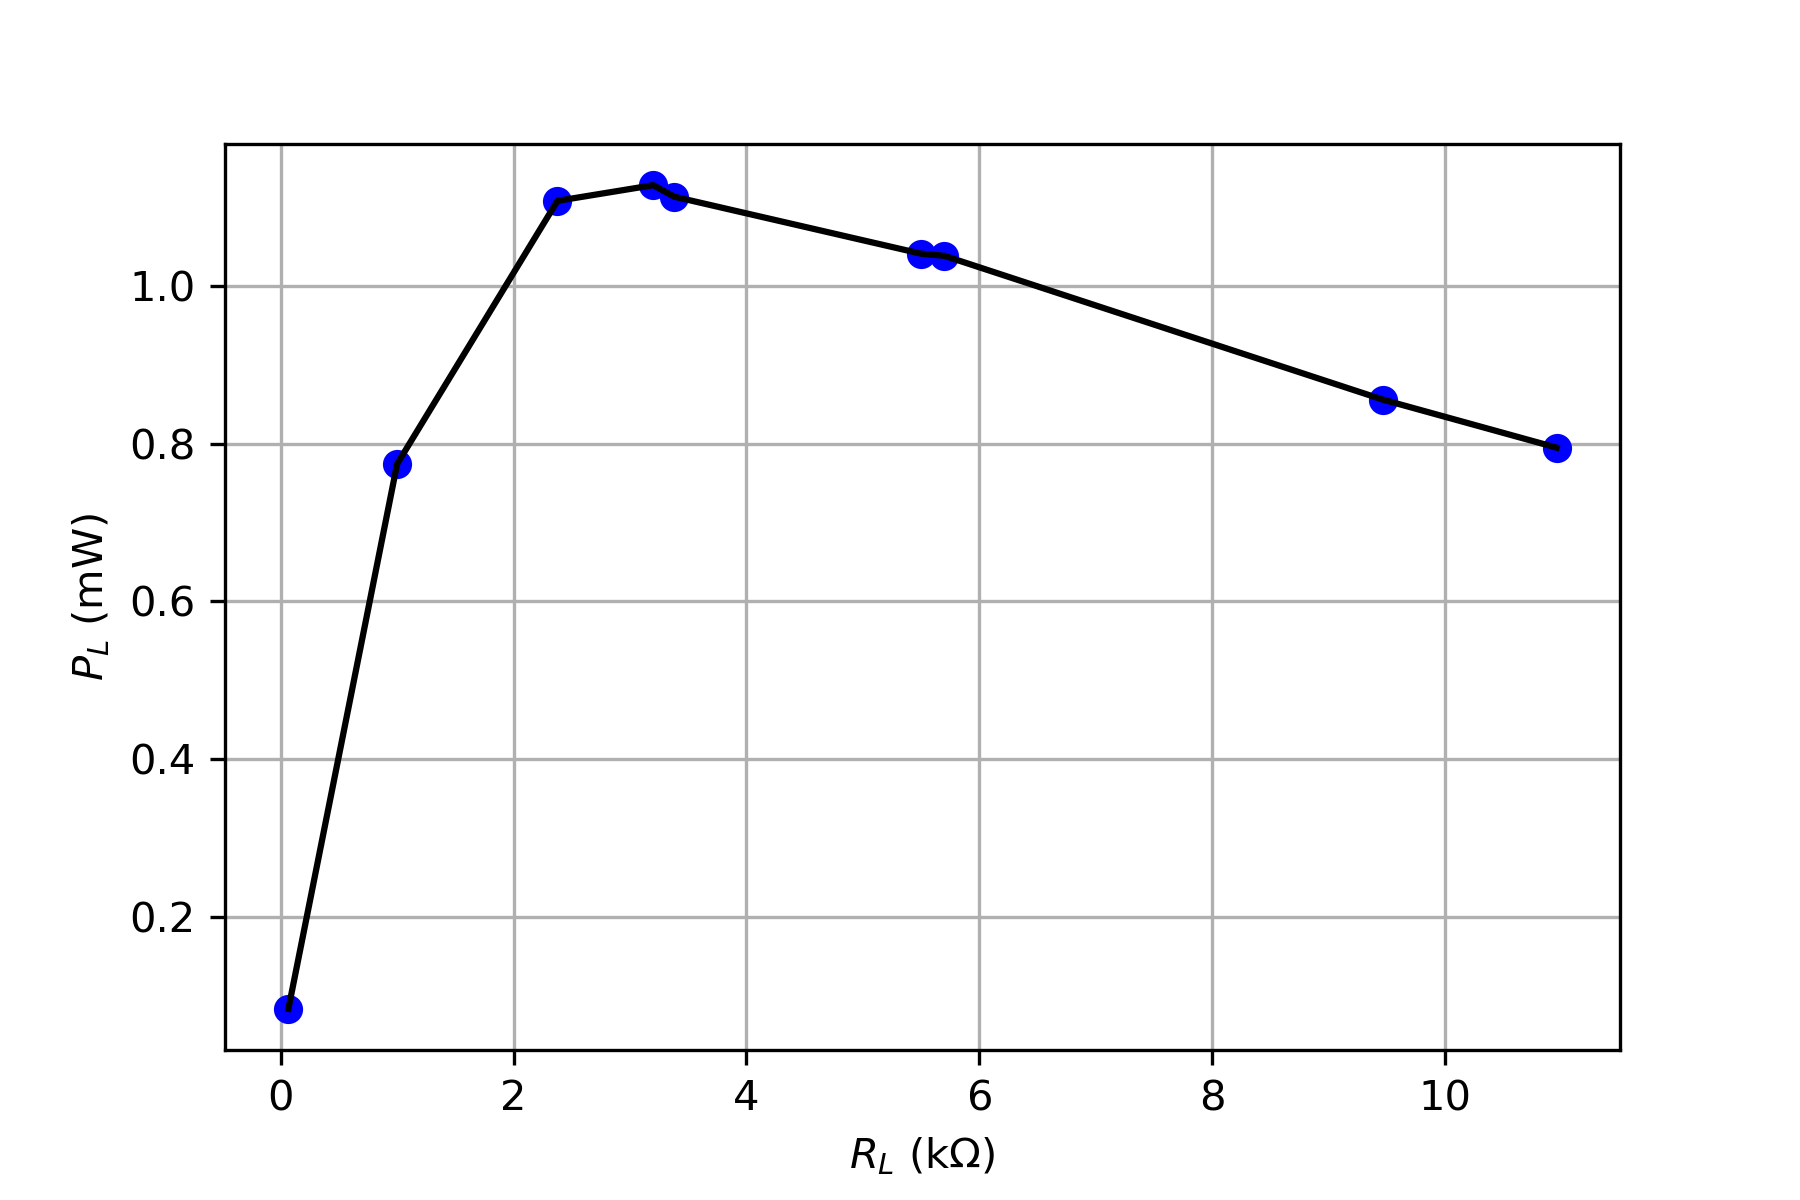
\includegraphics[scale=0.7]{ksken.png}
\end{figure}
El valor de $R_{L}$ para absorber la máxima resistencia es 3.366\,k$\Omega$.
\item \textbf{Calcular en cada caso el valor de la eficiencia $\bm{n}$.}\\
Los valores de la corriente y potencia por la fuente:
\begin{figure}[H]
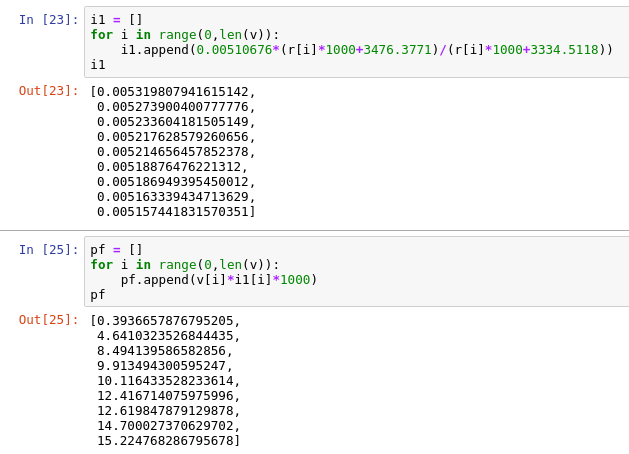
\includegraphics[scale=0.55]{kskenylaksmr.png}
\end{figure}
Los valores de $n$:
\begin{figure}[H]
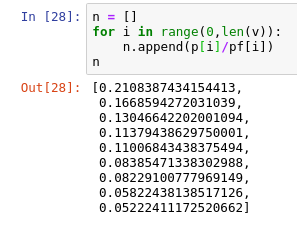
\includegraphics[scale=0.55]{kskenylaksmr2.png}
\end{figure}
\begin{figure}[H]
\centering
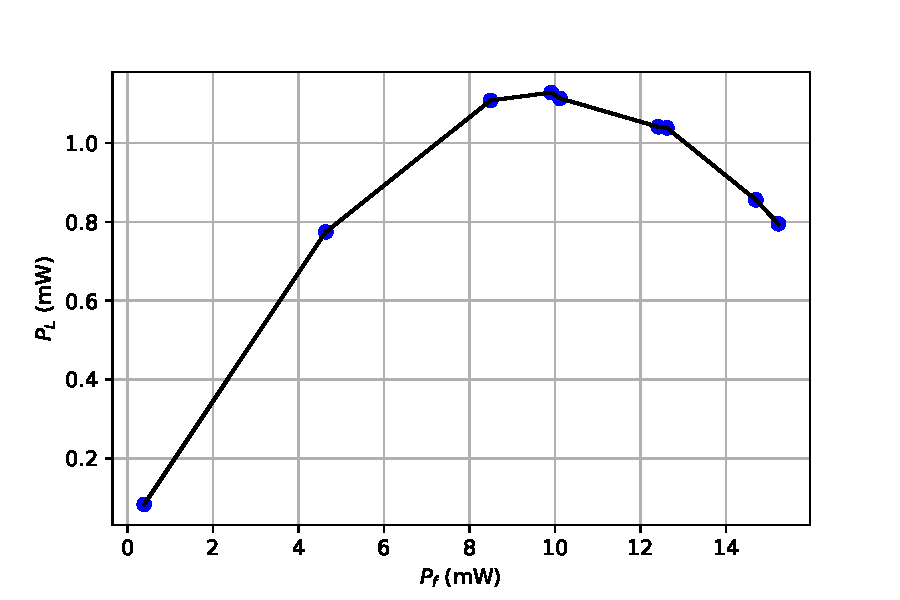
\includegraphics[scale=0.7]{vspotencia.pdf}
\caption{Potencia de la fuente vs Potencia de $R_{L}$}
\end{figure}
\item \textbf{Graficar $\bm{n \, \mathrm{vs} \, R_{L}}$ y determinar el valor de $\bm{n}$ correspondiente al valor de $\bm{R_{L}}$ que da la potencia máxima.}
\begin{figure}[H]
\centering
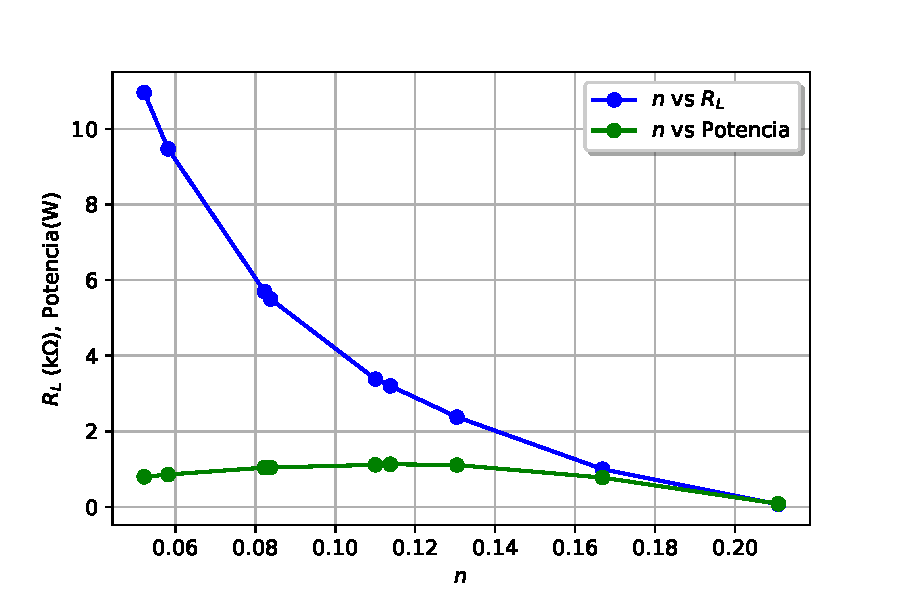
\includegraphics[scale=0.7]{vsnr.pdf}
\caption{$n$ vs $R_{L}$}
\end{figure}
El valor de $n$ para la máxima potencia corresponde a 0.110068.
\item \textbf{Comparar el valor de $\bm{R_{L}}$ obtenido gráficamente, que da la máxima potencia, con la resistencia que presenta la red pasiva entre los bornes CD.}\\
El $E_{th}$ es igual a 3.8443\,V, mientras que el $I_{No} = 0.001152$\,mA:
$$
R_{eq} = \frac{E_{th}}{I_{No}} = 3.334495\,\mathrm{k}\Omega
$$
Mientras que el valor hallado experimentalmente nos dice que $R_{eq} = 3.356\,\mathrm{k}\Omega$.
$$
\%\mathrm{Error\;relativo} = \frac{3.356-3.34495}{3.34495}\cdot 100\% = 0.64479\% 
$$
Mientras que $R_{L} = 3.366\,\mathrm{k}\Omega$
\item \textbf{Dar el circuito Thevenin equivalente de la red activa que alimenta $\bm{R_{L}}$ en el circuito utilizado, mostrando el valor de $\bm{R_{L}}$ que absorbe la máxima potencia, y $\bm{n}$}
\begin{figure}[H]
\centering
\begin{tikzpicture}[draw=DeepSkyBlue4,thin]
\tkzDefPoints{	0/0/A,
0/4/B,
3/4/C,
3/0/D,
7/4/E,
8/4/F,
8/0/G,
10/-0.5/H}
\draw[draw opacity=0, fill=yellow!30] (0,2) circle (.4);
\draw ({8,4}) to[R = 3.356\si{\kohm},color=Aquamarine4] (B) to[V=3.895V,color=red,thin] (A);
%\draw (C) to[R = 3.256\si{\kohm},color=Aquamarine4] (D);
\draw (A) to ({8,0});
\draw ({8,0}) to[R=$R_{L}\risingdotseq$3.366\si{\kohm},color=Aquamarine4] ({8,4});
%\draw (D) to ({10,0});
%\draw (C) to[R = 3.268\si{k\ohm},color=Aquamarine4] (E);
%\draw (E) to[R = 1.962\si{k\ohm},color=Aquamarine4] ({7,0});
%\draw (E) to[R = 1.968\si{\kohm},color=Aquamarine4] ({10,5});
%\draw ({10,5}) to[R = 3.366\si{\kohm},color=Aquamarine4] ({10,0});
%\draw (F) to[R = 193.3\si{\ohm},color=Aquamarine4] (G);
%\draw (G) to ({10,0});
%\draw ({10,0}) to (H) node[sground]{};
\end{tikzpicture}
\end{figure}
Con $n = 0.11$
\item \textbf{En un circuito con fuentes controladas, ¿cómo se obtiene la máxima potencia de transferencia? Demuestre.}\\
El teorema de máxima potencia nos dice:
$$
I_{L} = \frac{V_{th}}{R_{th} + R_{L}} \longrightarrow P_{L} = \left(\frac{V_{th}}{R_{th}+R_{L}}\right)^{2} \cdot R_{L}
$$
Derivando la expresión anterior:
$$
\frac{\mathrm{d}\, P_{L}}{R_{L}} = V_{th}^{2}\left( \frac{(R_{th}+R_{L})^{2}-2R_{L}(R_{th}+R_{L})}{(R_{th}+R_{L})^{4}} \right) \rightarrow R_{th}+R_{L} - 2R_{L} = 0 \longrightarrow R_{th} = R_{L}
$$
Lo que significa que, cuando $R_{th}=R_{L}$ la potencia se hace máxima. Entonces conocida la fuente de voltaje, se busca escoger una resistencia que sea igual a la resistencia equivalente del circuito de Thevenin para maximixar.
\end{enumerate}
\chapter{Conclusiones y recomendaciones}
\begin{enumerate}
\item Se concluye que el teorema de Thevenin y Norton son de gran utilidad para analizar cargas específicas variables sin la necesidad de modelar el circuito nuevamente.
\item Se recomienda verificar las conexiones previamente, sobretodo en el circuito 2 que fue más complejo.
\item Se concluye que la condición de máxima potencia para resistencias ocurre cuando está es igual a la resistencia equivalente de Thevenin y Norton.
\item Se concluye que los circuitos usados son lineales; es por ello que se cumplieron los teoremas. 
\end{enumerate}
\begin{thebibliography}{99}  %%%este es un contador para el número de bibliografías utilizados.
\addcontentsline{toc}{chapter}{Bibliograf\'{\i}a} %%% Para introducir la bibliografía en el índice.
%\bibitem{Rahman}{Rahman,Aminur y Doe, Hidekazu; ``Ion transfer of tetraalkylammonium cations at an interface between 
%frozen aqueous solution and 1,2-dichloroethane".{\em{Journal of Electroanalytical Chemistry}} {\bfseries 424},159,(1997).}
\bibitem{Gro}{Boylestad, Robert M. ``Introducción al análisis de circuitos''. {\em{Pearson}}}
\bibitem{Gro}{Sadiku, Matthew N. ``Fundamemtos de circuitos eléctricos''. {\em{Mc Graw Hill}}}
%\bibitem{Ding}{Ding, Zhifeng. ``Spectroelectrochemistry and photoelectrochemistry of charge transfer at liquid/liquid
%interfaces". {\em {Tesis, EPFL,}}(1999).}
%\bibitem{AL}{Alonso, Jose M. \em{Técnicas de mecanizado 1}}
%\bibitem{AL}{Alonso, Jose M. ``Técnicas de mecanizado 1". {\em{Paraninfo}} {\bfseries España-Madrid}, 6-20, (2001).}
%\bibitem{Samec2}{Samec Z., Lhotsky A., Jänchenová H., y Marecek, V. ``Interfacial tension and impedance measurements
%of interfaces between two inmiscible electrolyte solutions". {\em{Journal of Electroanalytical Chemistry}} {\bfseries
%43}, 47, (2000).}
%\bibitem{Day}{Day R.A. y Underwood A.L. {\textit{Química Analítica Cuantitativa}},5ºed. Prentice-Hall, México, 1998. 45-48.}
%\bibitem{Keyser}{Farah Abud, Michel. ``Determinación de la vida útil en herramientales de corte endurecido por el proceso de borurización en pasta''. {\em{Instituto tecnológico y de estudios superiores de Monterrey}}}
%\bibitem{Zolotorevski}{Escalona, I. ``Máquinas: herramientas por arranque de viruta.''.{\em{El Cid Editor.}}}
%\bibitem{Lasheras}{Lasheras. ``Tecnología de los Materiales Industriales''.} 
%\bibitem{Dieter}{Dieter. ``Metalurgia mecánica''.}
%\bibitem{Apraiz}{Apraiz, J. ``Tratamiento Térmico de los Aceros''.}
%\bibitem{Smith}{Smith, William F. y Ph.D. Hashemi, Javad ``Ciencia e ingeniería de materiales". {\em{
%Madrid: McGraw-Hill, Interamericana de España.}} 570, (2004).} 
%\bibitem{Callister}{Callister, William D. y Rethwisch, David G. ``Introducción a la ingeniería de los materiales''. %{\em{Barcelona Reverté.}}, 960, (2007).} 
%\bibitem{Askeland}{Askeland, Donald R., Pradeep P. Phulé y Wright, Wendelin J. ``Ciencia e ingeniería de los materiales''.{\em{México, D.F. Internacional Thomson Editores.}} {\textit{$6^{ta}$ edición}}, 1004, (2012).}
%\bibitem{HARDBANDING}{Tabla de conversión de escala de durezas. \begin{verbatim}http://%hardbandingsolutions.com/postle_sp/hardness.php
%\end{verbatim}}
%\bibitem{HE}{Fresadora. \begin{verbatim} http://lizdenbow.blogspot.com/
%\end{verbatim}}
%\bibitem{ASTM}{Normas ASTM.}
%\bibitem{NTP}{Normas NTP.}
\end{thebibliography}
\end{document}
